\documentclass{beamer}

\usepackage[czech, english]{babel}
\usepackage[utf8]{inputenc}	
\usepackage[square,sort,comma,numbers]{natbib}
\usepackage{textpos}

\usetheme{Malmoe}
\title{Zásuvný modul QGIS \\pro pozemní monitorování radiace}
\author{Michael Kala}
\date{29. června 2017}

\begin{document}

\begin{frame}
\titlepage
\end{frame}

\begin{frame}
\section{Úvod}
\frametitle{Zadání}

\begin{itemize}

	 

	\item Softwarový nástroj
	\item Odhad obdržené dávky gama záření na dané trase
	\item Státní ústav radiační ochrany, v.v.i.
	 
	

\end{itemize}
\end{frame}

\begin{frame}
\frametitle{Motivace}
\begin{itemize}
	\item Použití v praxi
	\item Předchozí spolupráce se SÚRO (Map corners coordinates)
	\item Programování
	
	
	
\end{itemize}
\end{frame}


\begin{frame}
\section{Pozemní monitorování radiace}
\frametitle{Pozemní monitorování radiace}
\begin{itemize}
	\item Ekvivalentní dávka a dávkový příkon (\textit{[Sv], [Sv/s]})
	\item Mobilní skupiny
	\item Radiační havárie
	\item Softwarový nástroj
		

\end{itemize}
\end{frame}

\begin{frame}
\section{Technologie}
\frametitle{Technologie}


	
	\begin{columns}
		\column{0.5\textwidth}
			\begin{figure}[H] \centering
				
\includegraphics[scale=0.12]{./pictures/qgis.png}
			\end{figure}
		\column{0.5\textwidth}
			\begin{figure}[H] \centering
				
\includegraphics[scale=0.3]{./pictures/python.png}

			\end{figure}
	\end{columns}
\begin{figure}[H] \centering	
	
\includegraphics[scale=0.035]{./pictures/pyqt.png}
\end{figure}
	


\end{frame}

\begin{frame}
\section{Zásuvný modul}
\frametitle{Zásuvný modul: Vstupní data}
\begin{columns}
	\column{0.5\textwidth} \centering
		\begin{itemize}
			\item Mapa dávkových příkonů
		\end{itemize}
	\column{0.5\textwidth} \centering
		\begin{itemize}
			\item Trasa monitorování
		\end{itemize}
\end{columns}
\begin{figure}[H] \centering	
	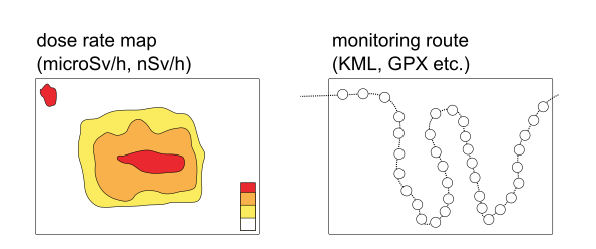
\includegraphics[scale=0.67]{./pictures/input.png}
\end{figure}

\end{frame}

\begin{frame}
\frametitle{Zásuvný modul: Výstupní data}
\begin{columns}

\column{0.5\textwidth}
	Zpráva o výpočtu (\textit{.txt}):
	\begin{itemize}
		\item Čas vytvoření zprávy
		\item Informace o trase
		\item Informace o části trasy bez dostupných dat
		\item Statistické hodnoty
		\item Nastavení
		\item Statický text
	\end{itemize}
\column{0.5\textwidth}
	\begin{figure}[H] \centering
		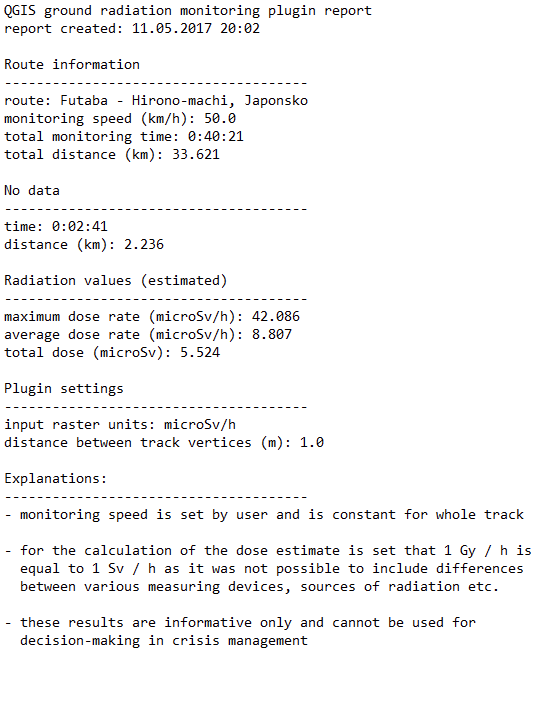
\includegraphics[scale=0.35]{./pictures/report.png}
	\end{figure}
\end{columns}


	
\end{frame}

\begin{frame}
\frametitle{Zásuvný modul: Výstupní data}

\begin{columns}

\column{0.5\textwidth}
	Soubor trasy (\textit{.shp}):
	\begin{itemize}
		\item Dávkový příkon
		\item Kumulativní čas
		\item Časový interval mezi body
		\item Kumulativní dávka

	\end{itemize}
\column{0.5\textwidth}
	\begin{figure}[H] \centering
		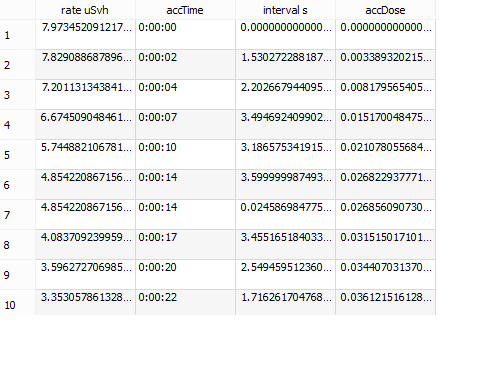
\includegraphics[scale=0.5]{./pictures/shapefile.png}
	\end{figure}
\end{columns}


\end{frame}

\begin{frame}
\frametitle{Zásuvný modul: Výstupní data}

Soubor s údaji o trase (volitelné, \textit{.csv}):

	\begin{figure}[H] \centering
		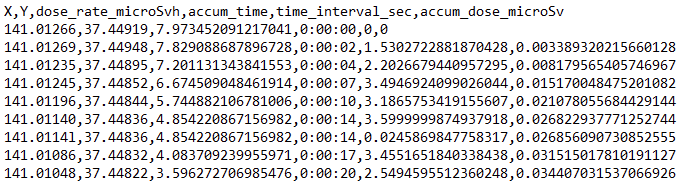
\includegraphics[scale=0.5]{./pictures/csv.png}
	\end{figure}



\end{frame}

\begin{frame}
\frametitle{Zásuvný modul: GUI}
\begin{columns}
	\column{0.5\textwidth}
	\begin{itemize}
		\item Hlavní okno
	\end{itemize}
\begin{figure}[H] \centering
		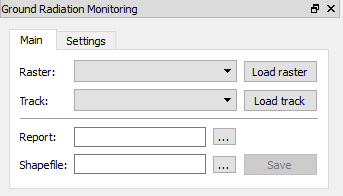
\includegraphics[scale=0.55]{./pictures/gui_main.png}
\end{figure}

	\column{0.5\textwidth}
	\begin{itemize}
		\item Nastavení
	\end{itemize}
\begin{figure}[H] \centering
		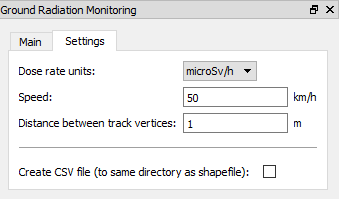
\includegraphics[scale=0.55]{./pictures/gui_settings.png}
\end{figure}


	
\end{columns}
\end{frame}

\begin{frame}
\frametitle{Zásuvný modul: Řešení}

\begin{itemize}
	\item Vzorkování trasy
	\item Extrakce hodnot rastru
	\item Výpočet
	\item Zápis do souborů
	\item Testování, připomínky
\end{itemize}



\end{frame}

\begin{frame}
\section{Závěr}
\frametitle{Závěr}
\begin{itemize}
	\item Rozšíření nástrojové sady SÚRO
	\item Zdrojový kód: \texttt{https://github.com/ ctu-geoforall-lab-projects/bp-kala-2017}
	\item Dokumentace 
	\item Licence GNU GPL
	\item Plán do budoucna
	


	%Shrnutí (rekapitulace - co vzniklo, co je můj přínos, vznikl tento program, který se může používat takto a takto) Plán do budoucna - rozšíření o vlastní plánování trasy, v čem by se dal modul ještě použít, osobní závěr (poděkování za vstřícnost ústavu, za vedení atd.), co mi to dalo odborně 
\end{itemize}
\end{frame}

\begin{frame}
\Huge{\centerline{Děkuji za pozornost.}}


\end{frame}

\begin{frame}
\frametitle{Otázky a odpovědi}
Plugin je pouze v angličtině - je v plánu i překlad do češtiny?
\begin{itemize}
\end{itemize}
	% Angličtina byla volena zejména kvůli možnosti využití nástroje i jinými - i zahraničními - institucemi nebo uživateli. Překlad do češtiny zatím plánovaný není, ale pokud by byl na vznešen požadavek na jazykovou lokalizaci, myslím, že by překlad zabral jeden večer.

\end{frame}

\begin{frame}
\frametitle{Otázky a odpovědi}
Je plugin omezen na konkrétní verze QGISu?
\end{frame}

\begin{frame}
\frametitle{Otázky a odpovědi}
Aktuálně vyžaduje plugin rastrová data ve stejném souřadnicovém systému jako plánovanou trasu (tj. WGS84 - EPSG:4326). Bylo by technicky realizovatelné přidat v případné budoucí verzi podporu i pro rastry v jiném souřadnicovém systému - např. UTM?
\end{frame}

\end{document}